\section{Throwing Booth}
\label{sec:booth}
The booth is constructed from Item aluminium profiles.
The background of the images shall remain the same, regardless of the current location.
Therefore, a white side wall opposite the camera is used.
When creating the booth design, care was taken to ensure that the size corresponds to the width of a table (\SI{750}{mm}).
This also defined the distance between the camera and the side wall.
With the opening angle of the lens, the minimum required size of the rear wall can be calculated as in equation \ref{eq:Fieldwith}. 
This size is called field of view.

\begin{equation}
	f_\text{w} = 2 \cdot a \cdot \tan\left( \frac{\vartheta}{2}\right) = \SI{690}{mm}
	\label{eq:Fieldwith}
\end{equation}

\begin{tabular}{rl}
	$f_\text{w} =$ & width of the field of view \\
	$a =$ & distance camera to side panel = \SI{630}{mm} \\
	$\vartheta =$ & horizontal angle of view = \SI{57.4}{\degree} \cite{baumer_lense} \\
\end{tabular}

%Whereby the following applies:
%\begin{itemize}
%	\item $f_\text{w}$ = width of the field of view
%	\item $a$ = Distance camera to back panel = \SI{630}{mm}
%	\item $\vartheta$ = horizontal angle of view = \SI{57.4}{\degree} \cite{baumer_lense}
%\end{itemize}

Given that the picture format is 1280 $\times$ \SI{1024}{px}, the height of the field of view $f_\text{h}$ is equal to

\begin{equation}
	f_\text{h} = f_\text{w} \cdot \frac{\SI{1024}{px}}{\SI{1280}{px}} = \SI{552}{mm}.
	\label{eq:Fieldhight}
\end{equation}

The objects should be thrown as far away from the camera as possible to be able to take more pictures per throw.
To ensure that the objects are thrown through the field of view and as far away from the camera as possible, there is a hole in the rear wall as a target.
It is located on the right side of the rear wall, which is further away from the camera.
If the objects are shot through the hole in the rear wall, they end up in a net.

The rear panel is made of a \SI{5}{mm} thick ABS plate.
This material is robust and withstands the impacts of the throwing objects.
The side wall is made of foamed PVC.
Due to the manufacturing process, the plate is less smooth, which results in less light reflections and therefore better pictures.
The drawings of the two plates can be found in appendix \ref{app:drawings_rear_panel} and \ref{app:drawings_side_panel}.

The whole throwing booth is drawn in the CAD tool Inventor. It is designed with all its components using a 3D model.
The camera is mounted on an Item profile with an aluminum mounting adapter which is shown in figure \ref{fig:mounting_adapter} and protected from damage with an aluminum sheet.
Both components have slotted holes to allow fine adjustments during assembly.
The drawings of these parts can be found in appendix \ref{app:drawings_camera_protection} and \ref{app:drawings_mounting_adapter}.

\begin{figure}[h]
	\centering
	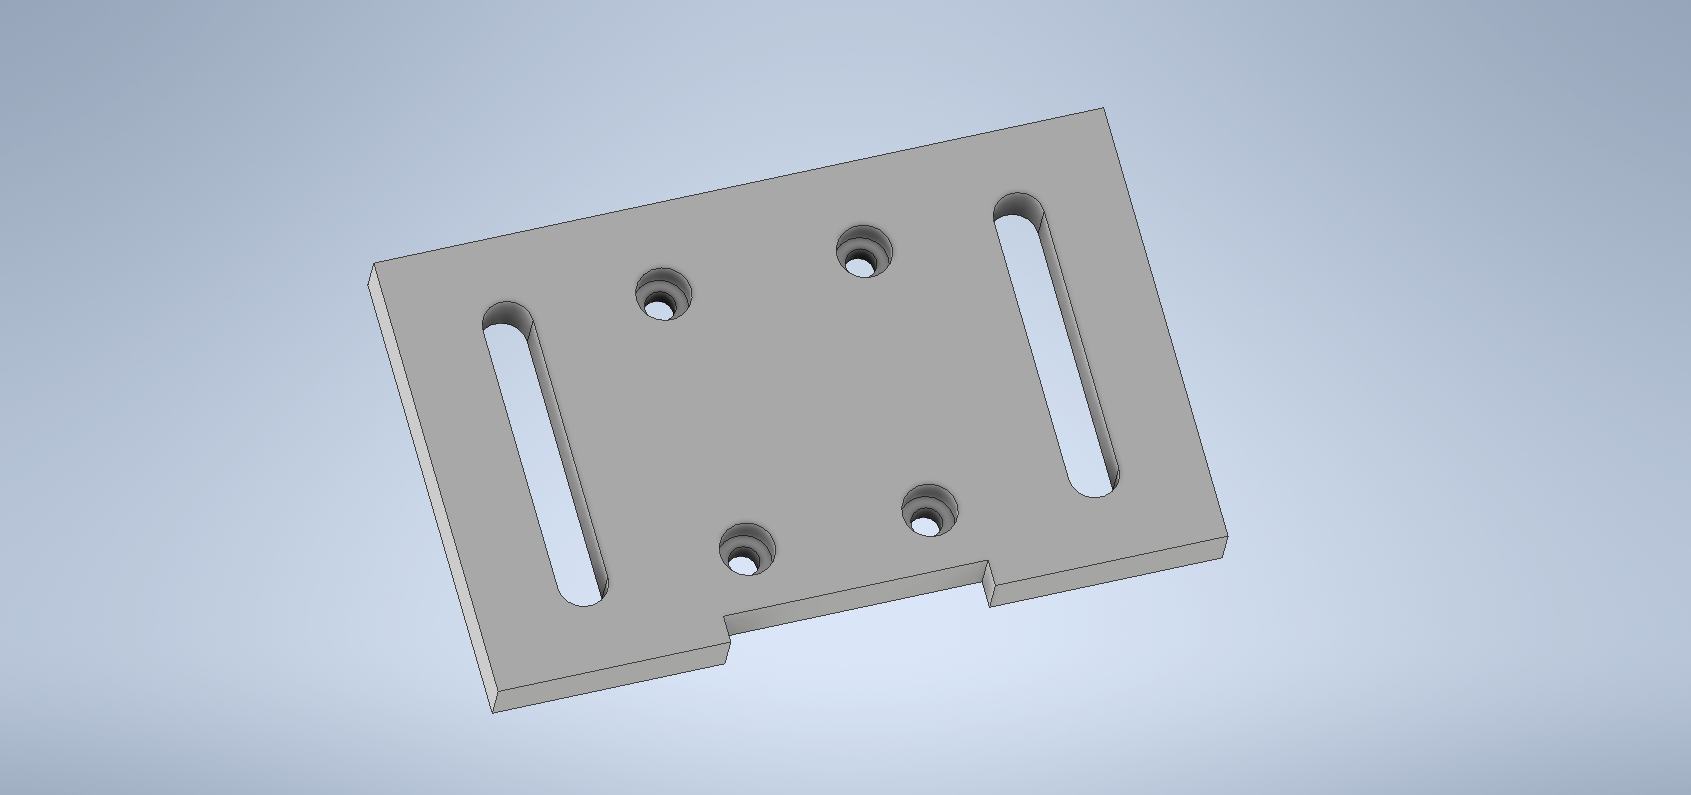
\includegraphics[width=0.4\textwidth]{graphics/mounting_adapter.png}
	\caption{Camera mounting adapter}
	\label{fig:mounting_adapter}
\end{figure}
\clearpage
The power supplies for all electronic components are placed in a box together with the Ultra96-V2.
The box is a case from Fibox with a transparent cover to give visitors an impression of the way it works.
It features a \SI{230}{VAC} power cable, a \SI{24}{VDC} output for lighting, a Mini DisplayPort cable for the monitor and the USB cable for the camera.
In addition, there are three fans on the walls to ensure that the Ultra96-V2 is cooled.
The box also contains terminal blocks and cable trunking to store cables that are too long.
Figure \ref{fig:fibox3d} shows a 3D model of the box. The construction drawings for the Fibox case can be found in appendix \ref{app:drawings_fibox_bottom}.

\begin{figure}[h]
	\centering
	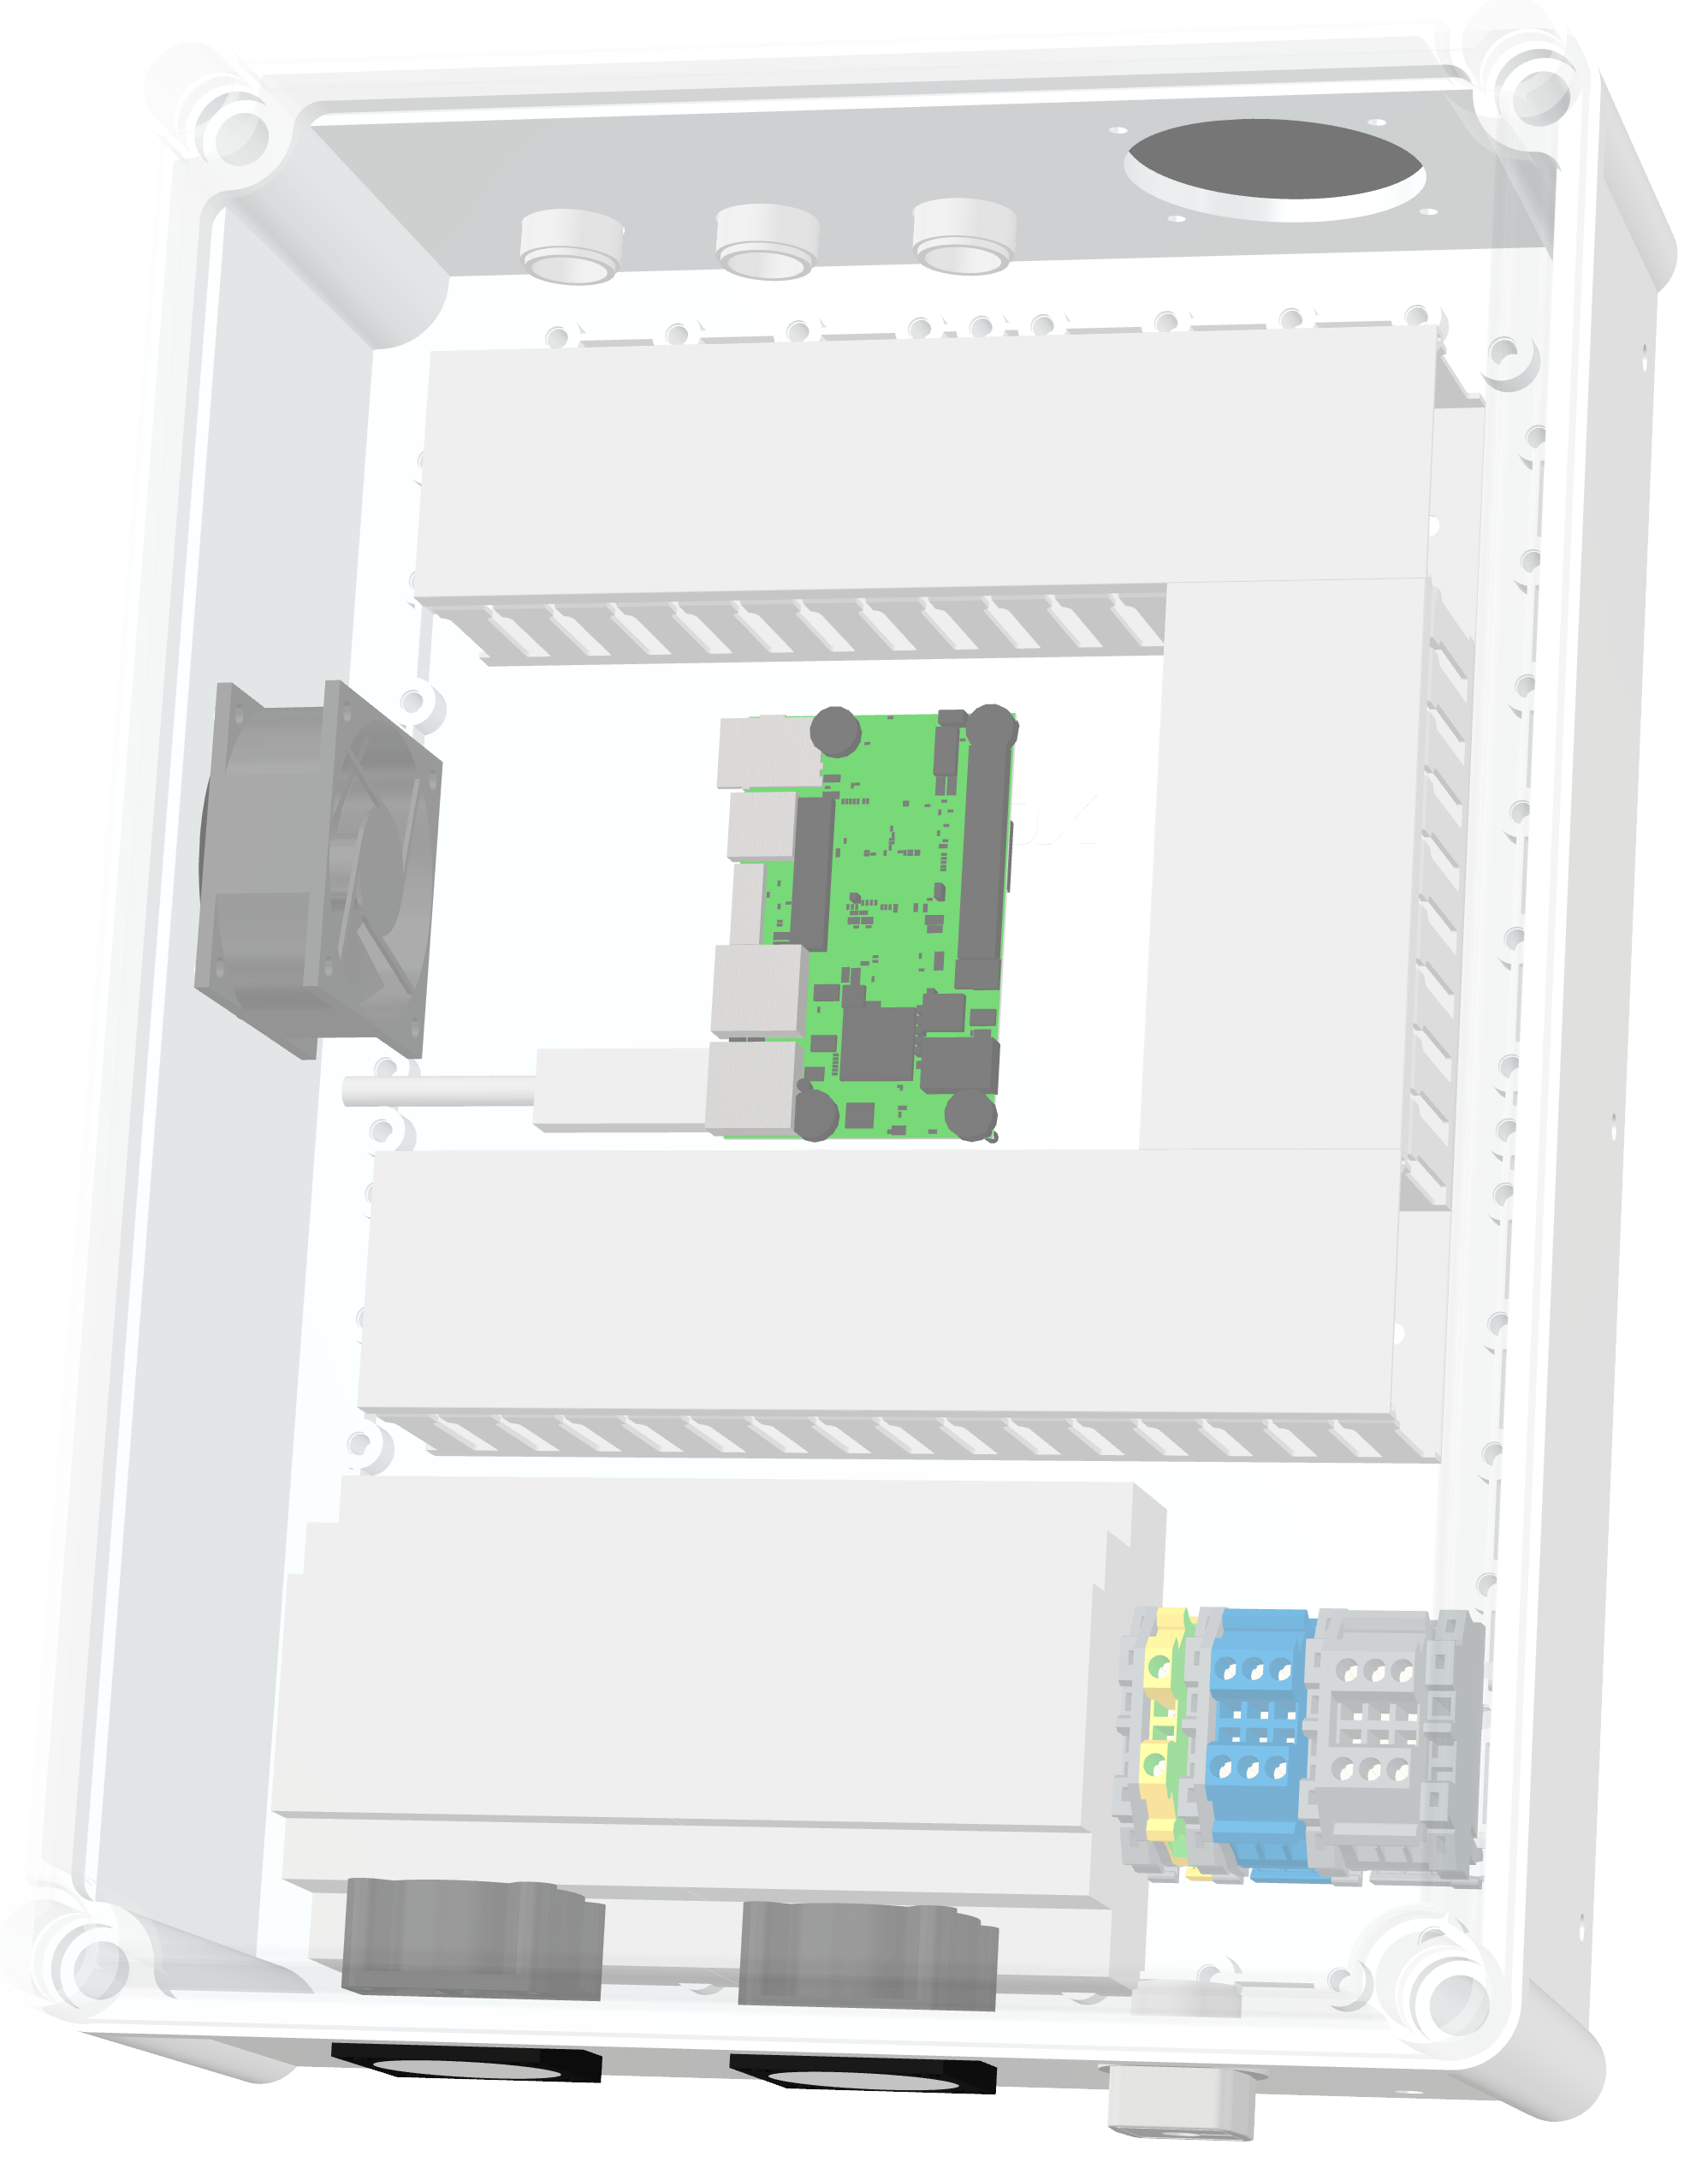
\includegraphics[width=0.6\textwidth]{graphics/case.png}
	\caption{3D model of the Fibox case}
	\label{fig:fibox3d}
\end{figure}
